\section{Average Vehicle Speed}
\label{sec:Results_MeanSpeed}

The mean vehicle speed as a function of \ac{mpr} is reported in Table~\vref{tab:MeanSpeed} and illustrated for three critical demand levels in Figures~\vref{fig:MeanSpeed_2077} through \vref{fig:MeanSpeed_3462}. The data reveals several key trends regarding the performance of the Standard, \ac{eco-glosa}, and \ac{flow-glosa} control strategies under the HBEFA4 and PHEMlight5 emission models.

\paragraph{Low to Intermediate Demand ($69$--$692~\unit{\veh\per\hour}$).}
In sub-saturated conditions, a consistent trend is the monotonic decrease in average speed under \ac{eco-glosa} as its \ac{mpr} increases, though the effect is mild. At the lightest load of $69~\unit{\veh\per\hour}$, the mean speed drops from $13.34~\unit{\metre\per\second}$ to $13.01~\unit{\metre\per\second}$ (a $2.5\%$ reduction) at $100\%$ \ac{mpr} with the HBEFA4 model. While \ac{eco-glosa} occasionally produces minor speed overshoots at very low \acp{mpr}, this gain is quickly negated as the controller's fuel-saving objective leads to more conservative speeds. In contrast, the \ac{flow-glosa} controller delivers consistent or slightly improved speeds relative to the Standard. At $69~\unit{\veh\per\hour}$, for instance, it improves the average speed by up to $4.1\%$ at $90\%$ \ac{mpr}.

\paragraph{Emerging Congestion ($1385$--$2077~\unit{\veh\per\hour}$).}
As demand increases, the negative impact of \ac{eco-glosa} on vehicle speeds becomes more pronounced. At a demand of $2077~\unit{\veh\per\hour}$, the degradation is significant; under the PHEMlight5 model, the average speed decreases from $12.46~\unit{\metre\per\second}$ at $0\%$ \ac{mpr} to $10.55~\unit{\metre\per\second}$ at $90\%$ \ac{mpr} (Figures~\vref{fig:MeanSpeed_HBEFA4_2077} and \vref{fig:MeanSpeed_PHEM_2077}). The \ac{flow-glosa} algorithm, however, continues to demonstrate flow stability, maintaining and progressively increasing speeds above the Standard baseline. At $2077~\unit{\veh\per\hour}$, it increases average speed from $12.46~\unit{\metre\per\second}$ to $12.88~\unit{\metre\per\second}$ at full penetration.

\begin{figure}[htbp]
  \centering
  \begin{subfigure}[b]{0.98\textwidth}
    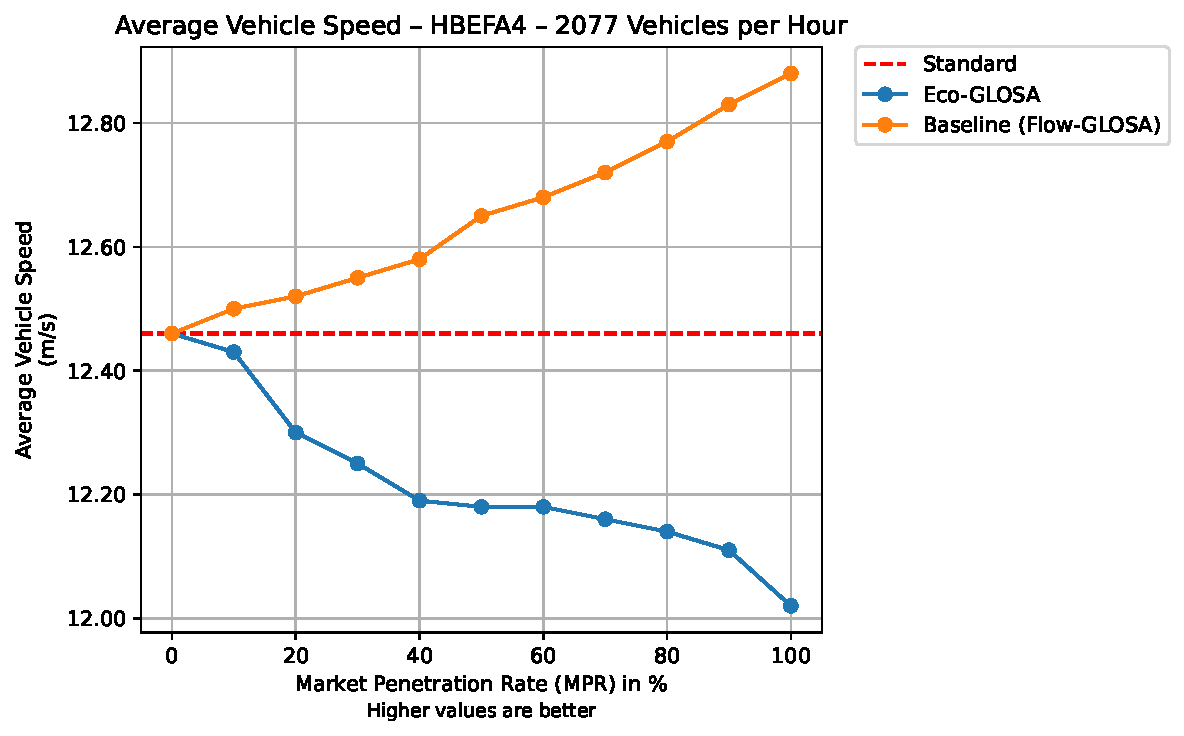
\includegraphics[width=\textwidth]{data/img/AverageVehicleSpeed/AverageVehicleSpeed_HBEFA4_Cars2077.pdf}
    \caption{Mean vehicle speed as a function of \ac{mpr} for the HBEFA4 emission model at a demand level of $2077\unit{\veh\per\hour}$.}
    \label{fig:MeanSpeed_HBEFA4_2077}
  \end{subfigure}
  \begin{subfigure}[b]{0.98\textwidth}
    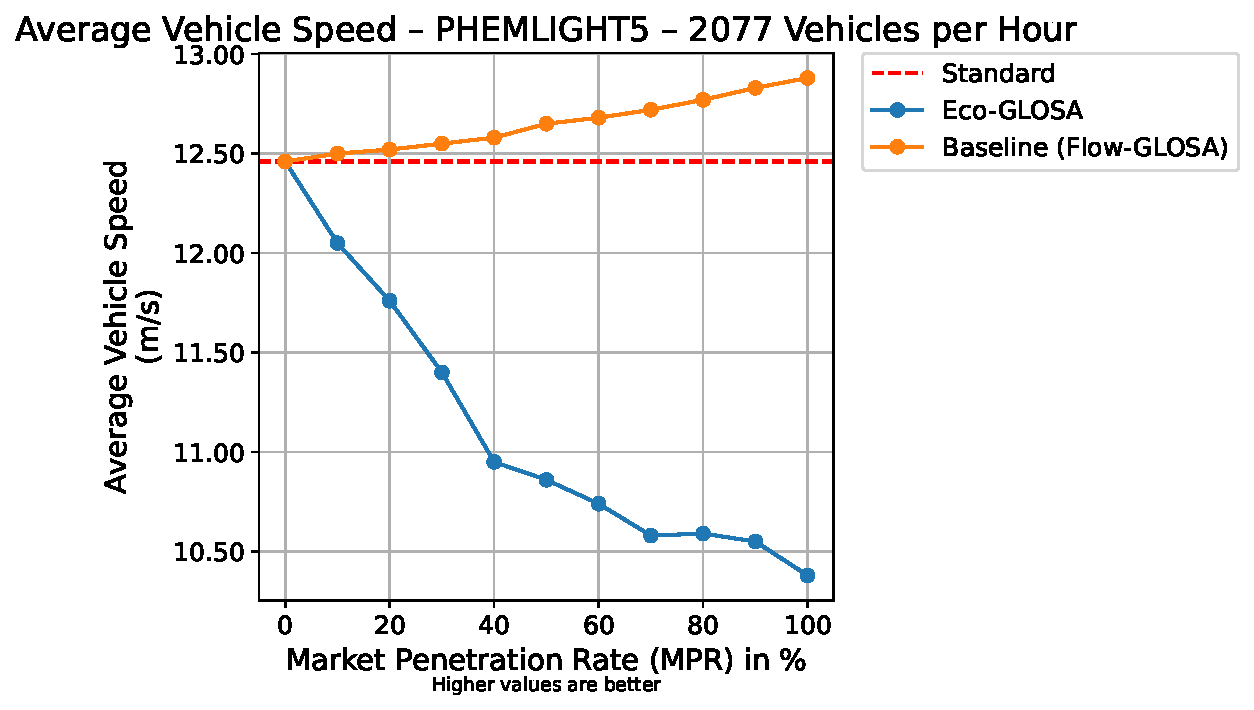
\includegraphics[width=\textwidth]{data/img/AverageVehicleSpeed/AverageVehicleSpeed_PHEMLIGHT5_Cars2077.pdf}
    \caption{Mean vehicle speed as a function of \ac{mpr} for the PHEMlight5 emission model at a demand level of $2077\unit{\veh\per\hour}$.}
    \label{fig:MeanSpeed_PHEM_2077}
  \end{subfigure}
  \caption[Mean speed vs. \ac{mpr} at $2077\unit{\veh\per\hour}$]{%
    Mean vehicle speed as a function of \ac{mpr} at a demand of $2077~\unit{\veh\per\hour}$. Both emission models (HBEFA4 and PHEMlight5) are compared under Standard, \ac{eco-glosa}, and \ac{flow-glosa} controllers.
  }
  \label{fig:MeanSpeed_2077}
\end{figure}

\paragraph{High Demand ($2769~\unit{\veh\per\hour}$).}
At this demand level, the system operates near its capacity limit, and clear breakpoints emerge where \ac{eco-glosa} can induce congestion, defined as speed falling below $4~\unit{\metre\per\second}$ (Figure~\vref{fig:MeanSpeed_2769}). The choice of emission model significantly dictates the system's stability. Under the transient-sensitive PHEMlight5 model, the network consistently degrades into a traffic jam when the \ac{mpr} reaches $30\%$. The HBEFA4 model, in contrast, exhibits high instability, characterised by significant speed fluctuations. The sharp speed drop observed at $60\%$ \ac{mpr} is an outlier that illustrates this fragility. This event is an instance of the cascading failure phenomenon described previously; in a single simulation run, persistently slow vehicles acting as a moving bottleneck can trigger a widespread, non-recoverable traffic jam. On the other hand, \ac{flow-glosa} manages to stay close to or even above Standard speeds across the entire \ac{mpr} range, showing that it is stable close to capacity.

\begin{figure}[htbp]
  \centering
  \begin{subfigure}[b]{0.98\textwidth}
    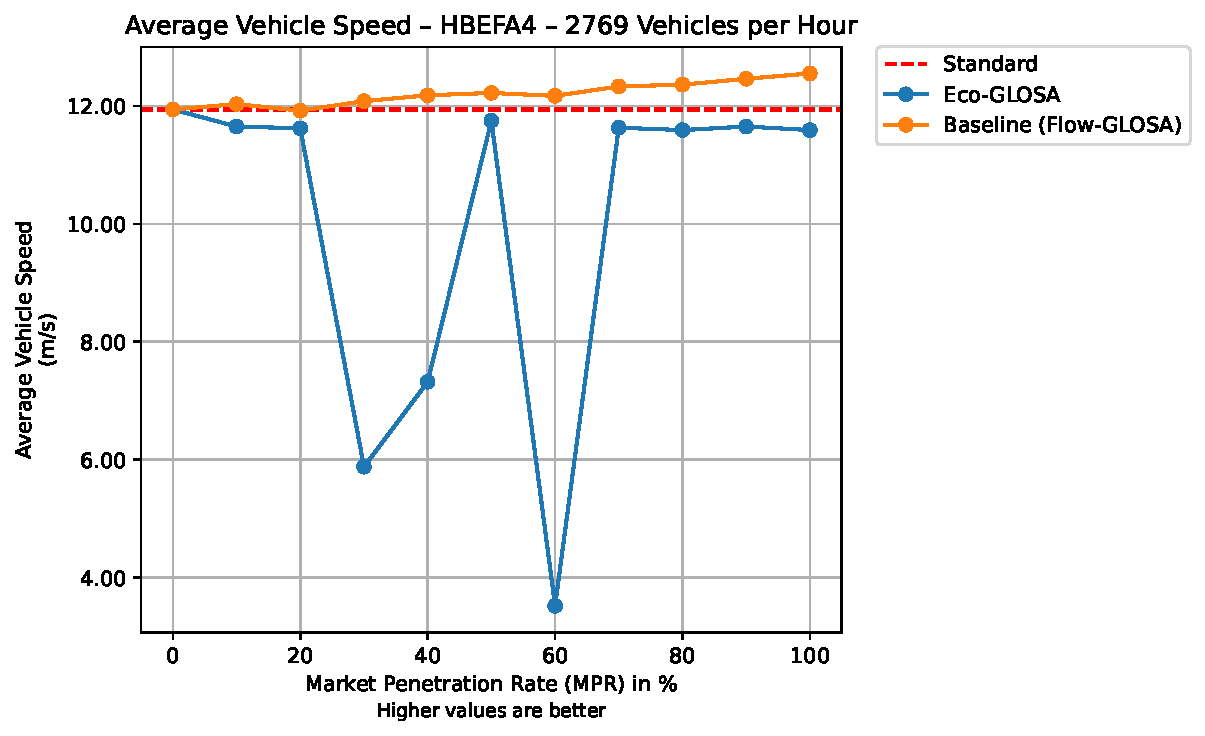
\includegraphics[width=\textwidth]{data/img/AverageVehicleSpeed/AverageVehicleSpeed_HBEFA4_Cars2769.pdf}
    \caption{Mean vehicle speed as a function of \ac{mpr} for the HBEFA4 emission model at $2769\,\mathrm{veh/h}$.}
    \label{fig:MeanSpeed_HBEFA4_2769}
  \end{subfigure}
  \begin{subfigure}[b]{0.98\textwidth}
    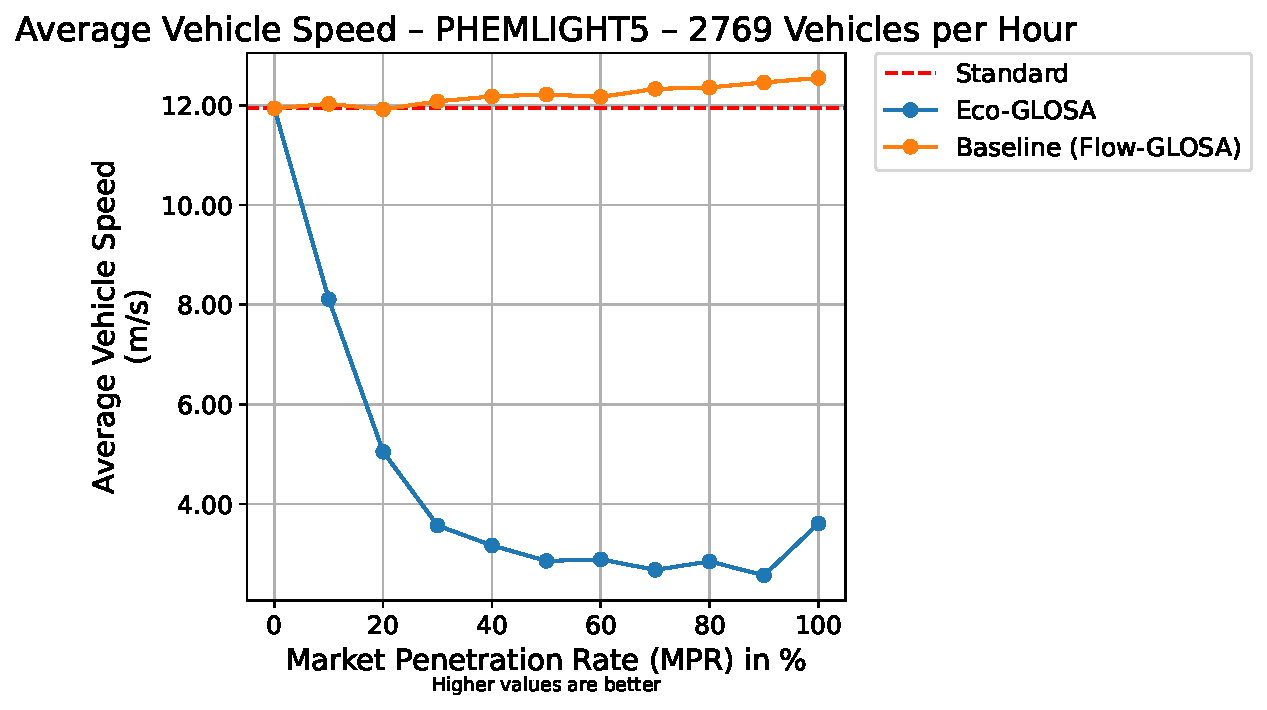
\includegraphics[width=\textwidth]{data/img/AverageVehicleSpeed/AverageVehicleSpeed_PHEMLIGHT5_Cars2769.pdf}
    \caption{Mean vehicle speed as a function of \ac{mpr} for the PHEMlight5 emission model at $2769\,\mathrm{veh/h}$.}
    \label{fig:MeanSpeed_PHEM_2769}
  \end{subfigure}
  \caption[Mean vehicle speed vs. \ac{mpr} at $2769~\unit{\veh\per\hour}$]{Mean vehicle speed versus \ac{mpr} at a congested demand of $2769~\unit{\veh\per\hour}$. The plots illustrate the performance divergence of the Standard, \ac{eco-glosa}, and \ac{flow-glosa} strategies under different emission models.}
\label{fig:MeanSpeed_2769}
\end{figure}

\paragraph{Saturated Regime ($3462~\unit{\veh\per\hour}$).}
Under fully saturated conditions, the network is already congested under the Standard scenario, with an average speed of only $3.86~\unit{\metre\per\second}$. The introduction of \ac{eco-glosa} not only fails to alleviate this breakdown, but further exacerbates the speed collapse across all penetration rates. Conversely, \ac{flow-glosa} proves capable of preventing the traffic jam once its penetration exceeds approximately $80\%$. As shown in Figures~\vref{fig:MeanSpeed_HBEFA4_3462} and \vref{fig:MeanSpeed_PHEM_3462}, it actively preserves free-flow conditions, with the mean speed increasing from the gridlocked $3.86~\unit{\metre\per\second}$ to $12.18~\unit{\metre\per\second}$ at $100\%$ \ac{mpr}.

\begin{figure}[htbp]
  \centering
  \begin{subfigure}[b]{0.98\textwidth}
    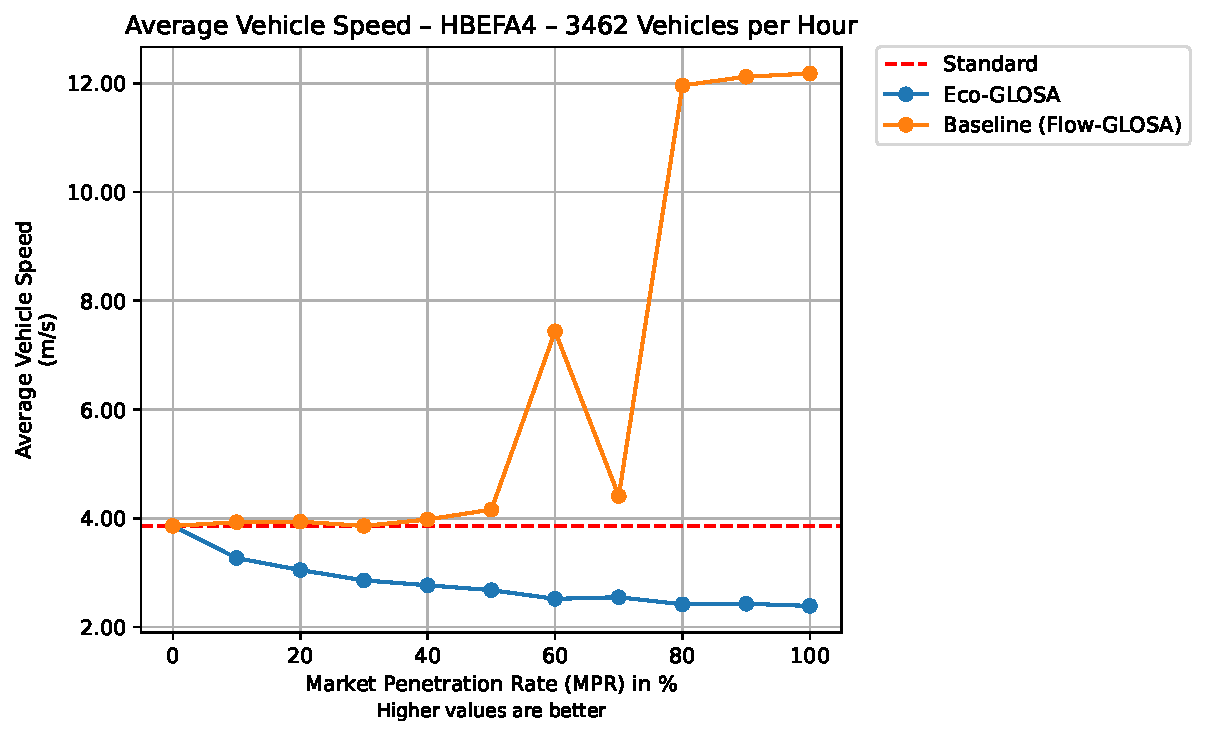
\includegraphics[width=\textwidth]{data/img/AverageVehicleSpeed/AverageVehicleSpeed_HBEFA4_Cars3462.pdf}
    \caption{Mean vehicle speed as a function of \ac{mpr} for the HBEFA4 emission model at $3462\,\mathrm{veh/h}$.}
    \label{fig:MeanSpeed_HBEFA4_3462}
  \end{subfigure}
  \begin{subfigure}[b]{0.98\textwidth}
    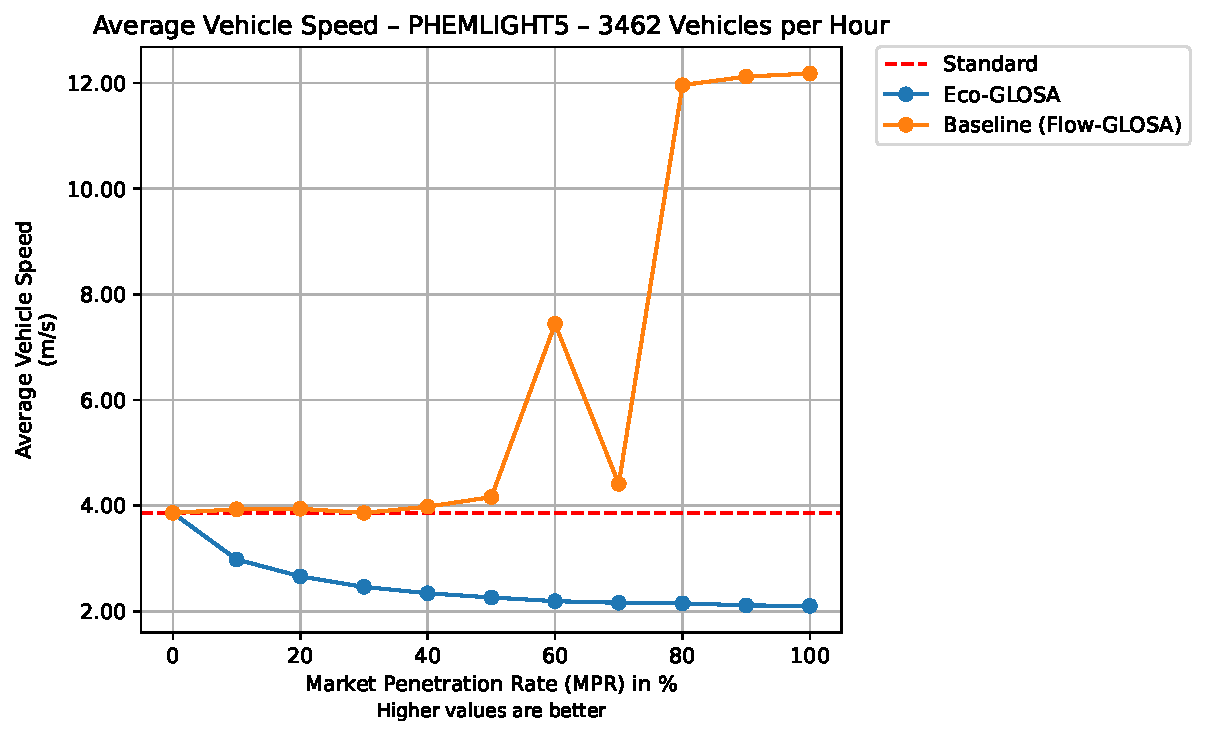
\includegraphics[width=\textwidth]{data/img/AverageVehicleSpeed/AverageVehicleSpeed_PHEMLIGHT5_Cars3462.pdf}
    \caption{Mean vehicle speed as a function of \ac{mpr} for the PHEMlight5 emission model at $3462\,\mathrm{veh/h}$.}
    \label{fig:MeanSpeed_PHEM_3462}
  \end{subfigure}
  \caption[Mean vehicle speed vs. \ac{mpr} at $3462~\unit{\veh\per\hour}$]{Mean vehicle speed as a function of \ac{mpr} in the fully saturated regime of $3462~\unit{\veh\per\hour}$. The results for the Standard, \ac{eco-glosa}, and \ac{flow-glosa} controllers are shown for both the HBEFA4 and PHEMlight5 models.}
\label{fig:MeanSpeed_3462}
\end{figure}

\paragraph{Implications.}
A primary distinction arises from the controllers' design philosophies. The advisory logic of \ac{flow-glosa} is purely kinematic, making its performance independent of the chosen emission model; its speed curves are identical for HBEFA4 and PHEMlight5. In contrast, the \ac{eco-glosa} controller's behaviour is intrinsically linked to the underlying fuel map. This sensitivity explains why, at high demand ($2769~\unit{\veh\per\hour}$), the system under the PHEMlight5 model consistently collapses into congestion at a low \ac{mpr} of $30\%$, while the HBEFA4 model only exhibits stochastic instability. This divergence occurs because the PHEMlight5 model more heavily penalises the short bursts of high engine power characteristic of stop-and-go traffic, prompting \ac{eco-glosa} to adopt even more conservative (slower) speed profiles.
\mynewline
This divergence becomes most critical in saturated conditions. At a demand of $3462~\unit{\veh\per\hour}$, \ac{eco-glosa}'s focus on individual vehicle efficiency is counterproductive, exacerbating existing gridlock. The \ac{flow-glosa} controller, however, proves its utility not merely as an efficiency tool but as a network resilience strategy. It successfully prevents the queue once the \ac{mpr} exceeds $80\%$, actively keeping free-flow conditions to a network that would otherwise remain gridlocked.
\mynewline
The granular comparison in Tables~\vref{tab:avg_speed_hbefa4} and \vref{tab:avg_speed_phemlight5} and Figure~\vref{fig:MeanSpeed_Combined} sharpens these implications from a user-centric perspective. An individual driver using \ac{eco-glosa} accepts a direct trade-off: potential fuel savings at the cost of a slower journey compared to non-equipped vehicles. This personal speed penalty, which can exceed $13\%$ under the PHEMlight5 model, may hinder user adoption. Conversely, the \ac{flow-glosa} system confers a direct benefit on its users, who consistently match or exceed the speeds of their unequipped peers. This aligns individual incentives with system-wide goals, making it a more compelling proposition for drivers. Therefore, deployment strategies must weigh the marginal fuel benefits of \ac{eco-glosa} in light traffic against its significant risk of causing network collapse under heavy load --- a risk not present with the throughput-oriented \ac{flow-glosa}.

\begin{figure}[htbp]
  \centering
  \begin{subfigure}[b]{0.98\textwidth}
    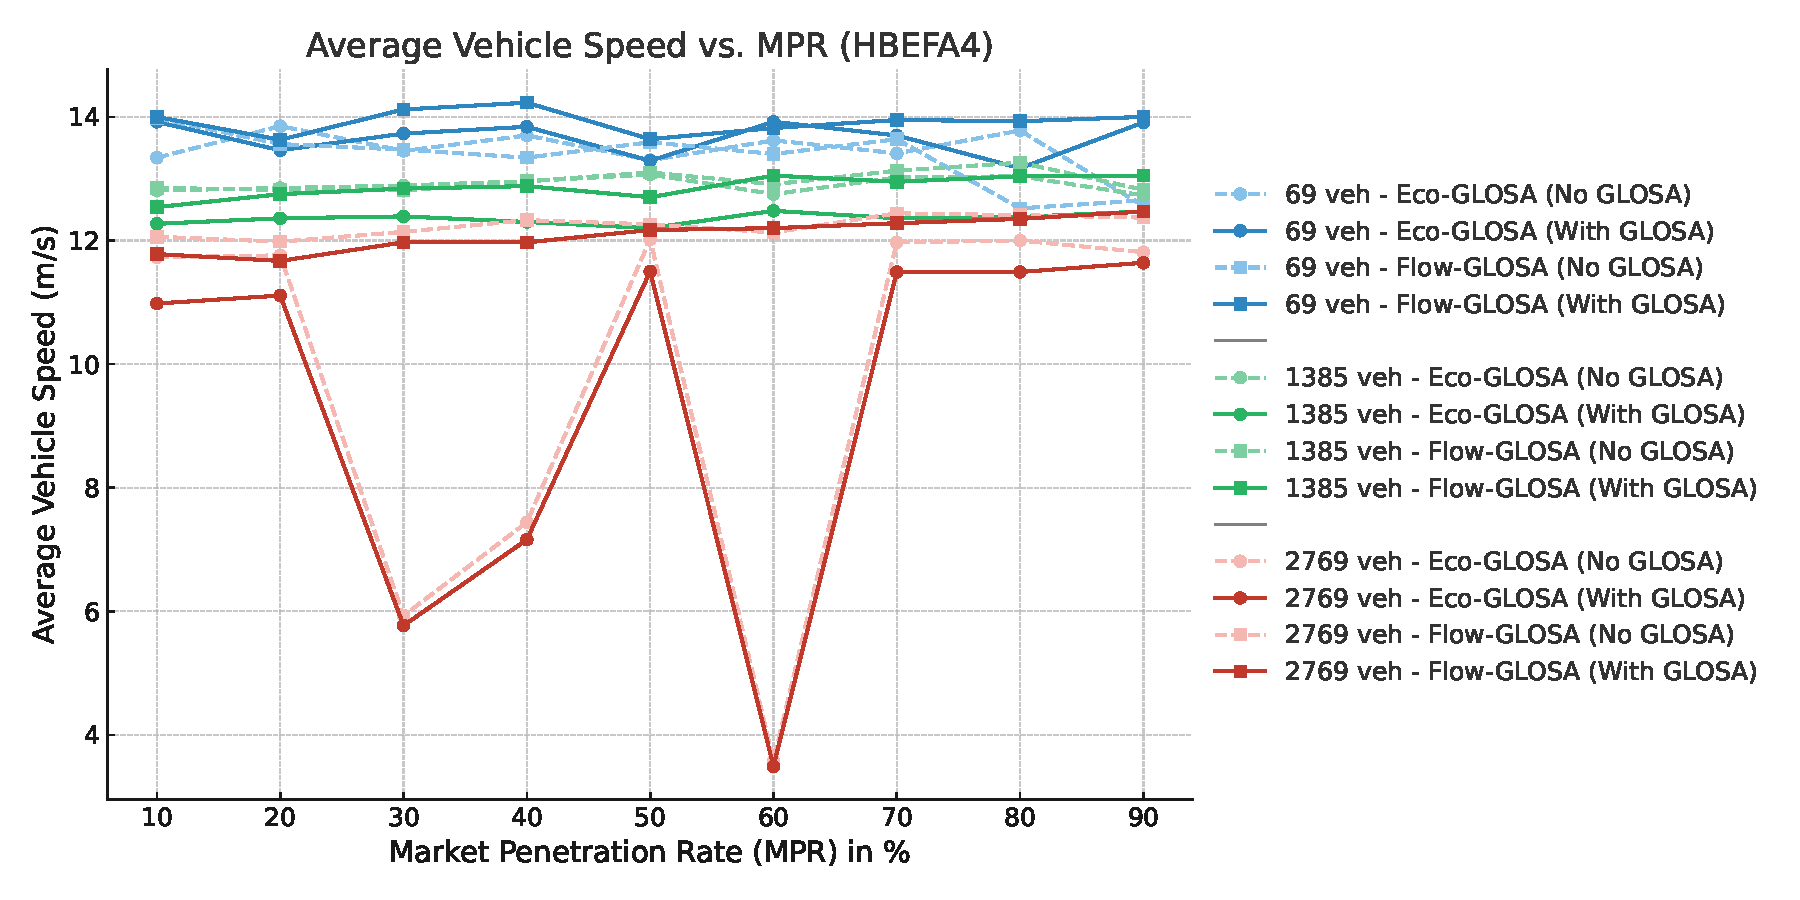
\includegraphics[width=\textwidth]{data/img/AverageVehicleSpeed/AvgSpeedHBEFA4Combined.pdf}
    \caption{Mean vehicle speed vs. \ac{mpr} for the HBEFA4 emission model.}
    \label{fig:MeanSpeed_HBEFA4_all}
  \end{subfigure}
  \begin{subfigure}[b]{0.98\textwidth}
    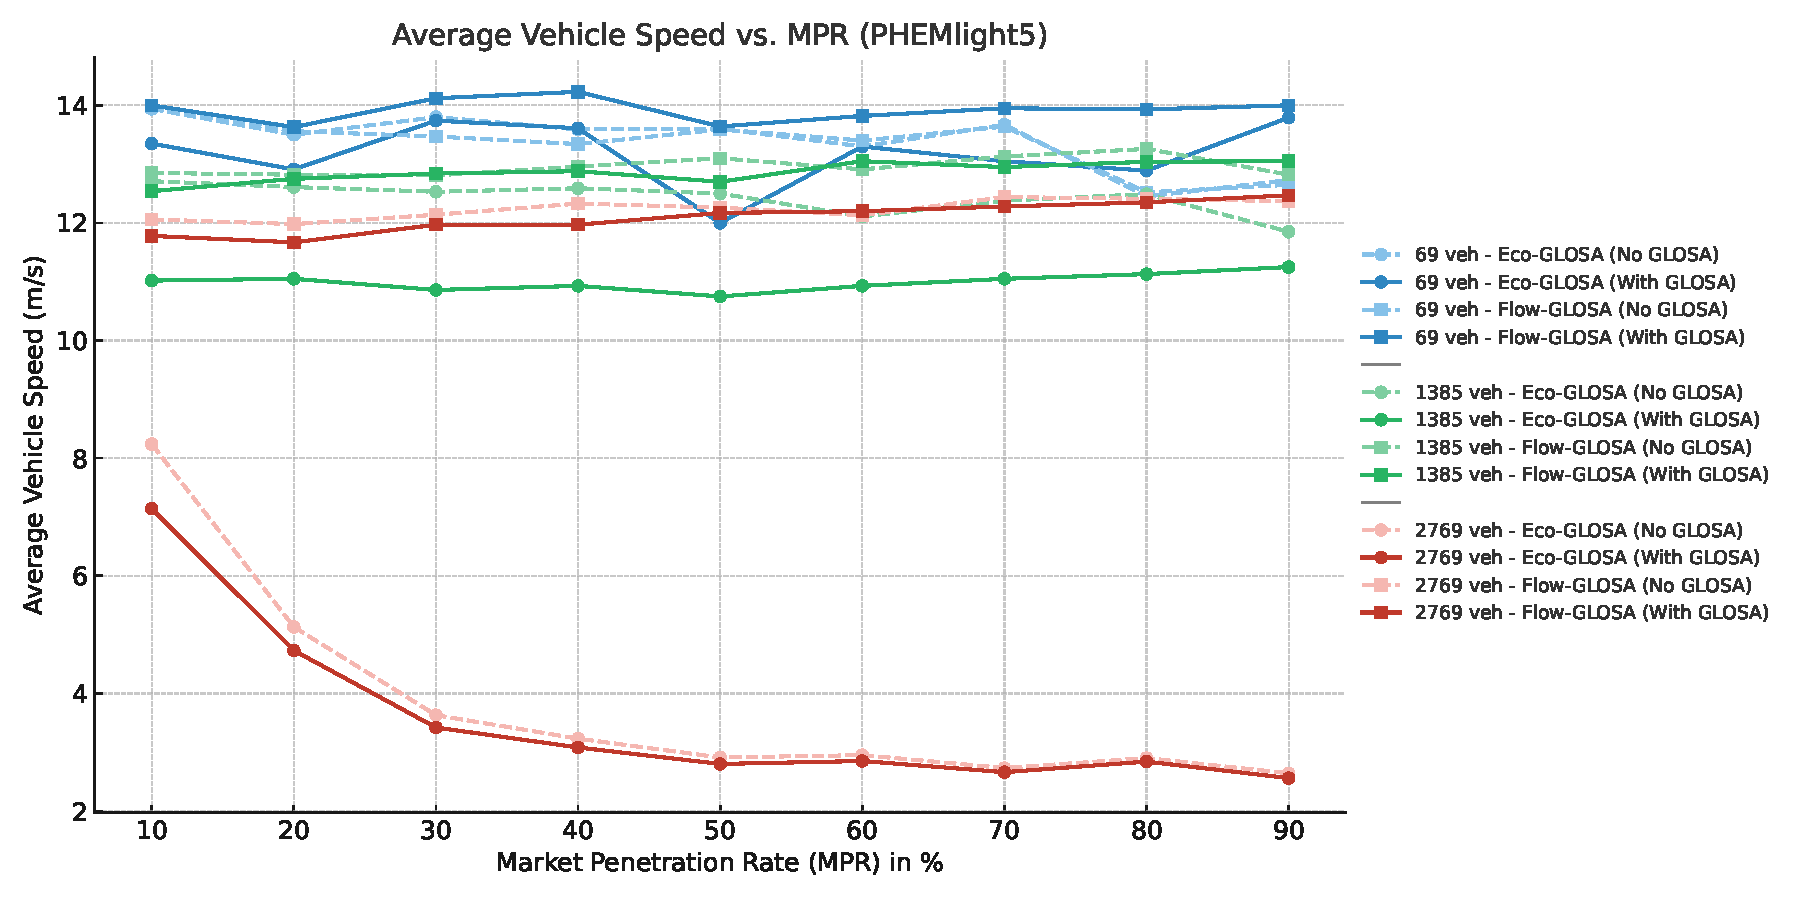
\includegraphics[width=\textwidth]{data/img/AverageVehicleSpeed/AvgSpeedPHEMlight5Combined.pdf}
    \caption{Mean vehicle speed vs. \ac{mpr} for the PHEMlight5 emission model.}
    \label{fig:MeanSpeed_PHEM_all}
  \end{subfigure}
  \caption[Mean vehicle speed vs. \ac{mpr} for both emission models]{Mean vehicle speed as a function of \ac{mpr} for both emission models, excluding the $0\%$ and $100\%$ \acp{mpr} (these are discarded since one of the speeds would be zero).}
  \label{fig:MeanSpeed_Combined}
\end{figure}

\paragraph{Key Takeaways.}
\begin{enumerate}
    \item \textbf{\ac{eco-glosa} Impact:} The average vehicle speed under \ac{eco-glosa} control consistently decreases as its market penetration rate increases. This effect is negligible at low demands but leads to significant speed degradation, network instability, and consequently congestion at high demands.
    \item \textbf{\ac{flow-glosa} Impact:} The \ac{flow-glosa} controller maintains or progressively improves average vehicle speeds across all traffic volumes and penetration rates. Crucially, it demonstrates the ability to prevent existing traffic jams in saturated conditions.
    \item \textbf{Emission Model Sensitivity:} The performance of \ac{eco-glosa} is highly sensitive to the underlying emission model. The more detailed PHEMlight5 model penalises transient states more heavily, causing \ac{eco-glosa} to advise more conservative speeds and inducing congestion at lower demand levels than the HBEFA4 model.
    \item \textbf{Congestion Thresholds:} \ac{eco-glosa} actively contributes to traffic breakdown when demand is high. For corridors operating near or above capacity (e.g., $> 2000~\unit{\veh\per\hour}$), a flow-oriented strategy is essential to maintain stability and prevent collapse.
    \item \textbf{User Perspective:} \ac{eco-glosa} imposes a speed penalty on its users in exchange for fuel efficiency, which may hinder adoption. In contrast, \ac{flow-glosa} provides a direct speed benefit to its users, aligning individual and system-wide goals.
\end{enumerate}

\begin{table}[htb]
  \centering
  \caption[Summary of mean vehicle speed by demand and \ac{mpr}]{A comprehensive summary of mean vehicle speed, in $\unit{\metre\per\second}$, tabulated by traffic demand and \ac{mpr}. The data compares the Standard (no \ac{glosa}), Baseline (\ac{flow-glosa}), and Eco (\ac{eco-glosa}) controller configurations.}
  \label{tab:MeanSpeed}
  \resizebox{\textwidth}{!}{%
  \begin{tabular}{r l l r *{10}{r}}
    \toprule
    Vehicles & Algorithm & Fuel & \textbf{0\% (Std)} & 10\% & 20\% & 30\% & 40\% & 50\% & 60\% & 70\% & 80\% & 90\% & 100\%\\
    \midrule
    69  & \ac{eco-glosa} & HBEFA4 & \textbf{13.34} & 13.86 & 13.45 & 13.71 & 13.51 & 13.46 & 13.71 & 13.72 & 13.05 & 13.81 & 13.01\\
    69  & Baseline (\ac{flow-glosa}) & HBEFA4 & \textbf{13.34} & 13.98 & 13.58 & 13.66 & 13.69 & 13.62 & 13.65 & 13.85 & 13.63 & 13.88 & 13.34\\
    69  & \ac{eco-glosa} & PHEMLIGHT5 & \textbf{13.34} & 13.89 & 13.38 & 13.79 & 13.60 & 12.77 & 13.30 & 13.23 & 12.81 & 13.70 & 12.34\\
    69  & Baseline (\ac{flow-glosa}) & PHEMLIGHT5 & \textbf{13.34} & 13.98 & 13.58 & 13.66 & 13.69 & 13.62 & 13.65 & 13.85 & 13.63 & 13.88 & 13.34\\
    \midrule
    138 & \ac{eco-glosa} & HBEFA4 & \textbf{13.24} & 13.51 & 13.29 & 13.46 & 13.56 & 13.36 & 13.52 & 13.17 & 13.12 & 13.01 & 12.97\\
    138 & Baseline (\ac{flow-glosa}) & HBEFA4 & \textbf{13.24} & 13.52 & 13.37 & 13.41 & 13.65 & 13.47 & 13.57 & 13.52 & 13.41 & 13.39 & 13.23\\
    138 & \ac{eco-glosa} & PHEMLIGHT5 & \textbf{13.24} & 13.38 & 13.40 & 13.36 & 13.64 & 13.15 & 13.39 & 13.03 & 12.99 & 12.70 & 12.50\\
    138 & Baseline (\ac{flow-glosa}) & PHEMLIGHT5 & \textbf{13.24} & 13.52 & 13.37 & 13.41 & 13.65 & 13.47 & 13.57 & 13.52 & 13.41 & 13.39 & 13.23\\
    \midrule
    346 & \ac{eco-glosa} & HBEFA4 & \textbf{13.24} & 13.24 & 13.14 & 13.07 & 13.18 & 13.01 & 13.08 & 13.04 & 12.96 & 12.99 & 12.87\\
    346 & Baseline (\ac{flow-glosa}) & HBEFA4 & \textbf{13.24} & 13.27 & 13.19 & 13.20 & 13.25 & 13.28 & 13.33 & 13.33 & 13.35 & 13.36 & \textbf{13.48}\\
    346 & \ac{eco-glosa} & PHEMLIGHT5 & \textbf{13.24} & 13.20 & 12.83 & 12.71 & 12.80 & 12.77 & 12.56 & 12.59 & 12.52 & 12.64 & 12.50\\
    346 & Baseline (\ac{flow-glosa}) & PHEMLIGHT5 & \textbf{13.24} & 13.27 & 13.19 & 13.20 & 13.25 & 13.28 & 13.33 & 13.33 & 13.35 & 13.36 & \textbf{13.48}\\
    \midrule
    692 & \ac{eco-glosa} & HBEFA4 & \textbf{13.17} & 13.13 & 13.17 & 13.09 & 13.04 & 13.01 & 13.05 & 12.94 & 12.91 & 12.82 & 12.81\\
    692 & Baseline (\ac{flow-glosa}) & HBEFA4 & \textbf{13.17} & 13.23 & 13.25 & 13.20 & 13.27 & 13.22 & 13.36 & 13.25 & 13.31 & 13.39 & 13.33\\
    692 & \ac{eco-glosa} & PHEMLIGHT5 & \textbf{13.17} & 13.08 & 12.95 & 12.71 & 12.68 & 12.52 & 12.49 & 12.38 & 12.24 & 12.11 & 12.10\\
    692 & Baseline (\ac{flow-glosa}) & PHEMLIGHT5 & \textbf{13.17} & 13.23 & 13.25 & 13.20 & 13.27 & 13.22 & 13.36 & 13.25 & 13.31 & 13.39 & 13.33\\
    \midrule
    1385 & \ac{eco-glosa} & HBEFA4 & \textbf{12.84} & 12.75 & 12.75 & 12.74 & 12.69 & 12.62 & 12.59 & 12.55 & 12.51 & 12.49 & 12.41\\
    1385 & Baseline (\ac{flow-glosa}) & HBEFA4 & \textbf{12.84} & 12.82 & 12.81 & 12.82 & 12.93 & 12.90 & 13.00 & 13.00 & 13.08 & 13.03 & 13.07\\
    1385 & \ac{eco-glosa} & PHEMLIGHT5 & \textbf{12.84} & 12.52 & 12.27 & 11.98 & 11.87 & 11.56 & 11.37 & 11.42 & 11.38 & 11.31 & 11.31\\
    1385 & Baseline (\ac{flow-glosa}) & PHEMLIGHT5 & \textbf{12.84} & 12.82 & 12.81 & 12.82 & 12.93 & 12.90 & 13.00 & 13.00 & 13.08 & 13.03 & 13.07\\
    \midrule
    2077 & \ac{eco-glosa} & HBEFA4 & \textbf{12.46} & 12.43 & 12.30 & 12.25 & 12.19 & 12.18 & 12.18 & 12.16 & 12.14 & 12.11 & 12.02\\
    2077 & Baseline (\ac{flow-glosa}) & HBEFA4 & \textbf{12.46} & 12.50 & 12.52 & 12.55 & 12.58 & 12.65 & 12.68 & 12.72 & 12.77 & 12.83 & 12.88\\
    2077 & \ac{eco-glosa} & PHEMLIGHT5 & \textbf{12.46} & 12.05 & 11.76 & 11.40 & 10.95 & 10.86 & 10.74 & 10.58 & 10.59 & 10.55 & 10.38\\
    2077 & Baseline (\ac{flow-glosa}) & PHEMLIGHT5 & \textbf{12.46} & 12.50 & 12.52 & 12.55 & 12.58 & 12.65 & 12.68 & 12.72 & 12.77 & 12.83 & 12.88\\
    \midrule
    2769 & \ac{eco-glosa} & HBEFA4 & \textbf{11.94} & 11.65 & 11.62 & \textbf{5.88} & \textbf{7.32} & 11.75 & \textbf{3.52} & 11.63 & 11.59 & 11.65 & 11.59\\
    2769 & Baseline (\ac{flow-glosa}) & HBEFA4 & \textbf{11.94} & 12.03 & 11.92 & 12.08 & 12.18 & 12.22 & 12.17 & 12.33 & 12.36 & 12.46 & 12.55\\
    \textbf{2769} & \textbf{\ac{eco-glosa}} & \textbf{PHEMLIGHT5} & \textbf{11.94} & \textbf{8.11} & \textbf{5.05} & \textbf{3.57} & \textbf{3.17} & \textbf{2.86} & \textbf{2.89} & \textbf{2.68} & \textbf{2.85} & \textbf{2.57} & \textbf{3.61}\\
    2769 & Baseline (\ac{flow-glosa}) & PHEMLIGHT5 & \textbf{11.94} & 12.03 & 11.92 & 12.08 & 12.18 & 12.22 & 12.17 & 12.33 & 12.36 & 12.46 & 12.55\\
    \midrule
    \textbf{3462} & \textbf{\ac{eco-glosa}} & \textbf{HBEFA4} & \textbf{3.86} & \textbf{3.27} & \textbf{3.05} & \textbf{2.86} & \textbf{2.77} & \textbf{2.68} & \textbf{2.52} & \textbf{2.55} & \textbf{2.42} & \textbf{2.43} & \textbf{2.39}\\
    3462 & Baseline (\ac{flow-glosa}) & HBEFA4 & \textbf{3.86} & 3.93 & 3.94 & 3.86 & 3.98 & 4.16 & \textbf{7.44} & 4.41 & \textbf{11.96} & \textbf{12.12} & \textbf{12.18}\\
    \textbf{3462} & \textbf{\ac{eco-glosa}} & \textbf{PHEMLIGHT5} & \textbf{3.86} & \textbf{2.98} & \textbf{2.66} & \textbf{2.46} & \textbf{2.34} & \textbf{2.26} & \textbf{2.19} & \textbf{2.16} & \textbf{2.15} & \textbf{2.11} & \textbf{2.10}\\
    3462 & Baseline (\ac{flow-glosa}) & PHEMLIGHT5 & \textbf{3.86} & 3.93 & 3.94 & 3.86 & 3.98 & 4.16 & \textbf{7.44} & 4.41 & \textbf{11.96} & \textbf{12.12} & \textbf{12.18}\\
    \bottomrule
  \end{tabular}
  }
\end{table}